%Chapter 3
In order to predict disorder from XANES spectra, we rely on machine learning, a technique capable of building highly non-linear models from a large collection of data. Due to the integral part of machine learning, specifically deep learning, this chapter serves as a basis for defining, first, how neural netorks fundementally work, and then the specific implimentations used in the project.

First we clarify the terms machine learning (ML), deep learning, and artificial intelligence (AI). Machine learning refers to the statistical technique of fitting a model to a large collection of data. These models can either be regressors or classifiers, the former being able to predict a continuous range of values and the latter being a discrete predictor. Neural networks are one example of a machine learning model that tends to be computationally intensive. They are useful for creating highly non-linear models capable of making difficult predictions and solving difficult tasks. Neural networks were inspired by biological processing systems, and the graphical representation includes common terms such as ``nodes'' and ``connections.'' The field of ML involving ANNs with many layers is referred to as deep learning \cite{schmidhuber2015deep}. AI is a subfield of deep learning where a neural network is trained to generate human-like responses, such as a chatbot or a virtual assistant. 

With these definitions, to predict disorder from XANES we utilize deep learning to train a regression-based neural network. The following sections will walk through the mathematical process of training a simple neural network. In practice, sophisticated APIs such as Google's TensorFlow or Facebook's PyTorch handle the mathematical backend; however, one should fundamentally understand what these frameworks are doing.
% \cite{tensorflow2015-whitepaper} 
% \cite{pytorch-paper}

\section{Feedforward and Backpropagation in ANNs}

Understanding how a neural network makes a prediction requires a solid grasp of linear algebra. The process where a NN passes information from the input to the subsequent layers to make a prediction is called the feedforward process. The name comes from the operation where each layer of the NN passes information to the next layer until the reaching output layer. The process of updating the weights of the NN is called backpropagation and relies principally on vector calculus. Neither action is particularly mathematically complicated; however, there are so many parts that it is easy to get lost in the sea of similar-sounding partial derivatives. In this next section, we explicitly walk through the math for the feedforward process of a fully connected (affine) neural network.

\subsection{Feedforward}
Consider the neural network in figure \ref{fig:simpleNN} with an input layer of three nodes, a single hidden layer with five nodes, and an output layer with two nodes. The input layer (zeroth layer) has a cardinality of $ \mu=3 $ and is represented in Einstein notation\footnote{Recall that in Einstein notation repeated indices are implicitly summed over.} as a row vector $ x_\mu $. Each edge in the graph represents a weight that is multiplied with the connected node on the left. Each node in the input layer is multiplied by the weight of the connected edge and added together. This operation for all input nodes and weights can thus be represented as a dot product between the input layer row vector and a weight matrix. The hidden layer (first layer) has a cardinality of $ \nu=5 $. Thus, the resulting dot product is $ x_\mu W_\nu^{\mu(1)} $ where $ W_\nu^{\mu(1)} $ represents the matrix of weights to create the first layer. While this result has the correct dimensionality for the hidden layer, there are still two operations reuired to produce the actual values for the nodes $ h_\nu^{(1)} $. First, a small trainable parameter, $ b_\nu $  is added to every value from the previous calculation. The values in this row vector are called biases and are introduced to prevent overfitting ---i.e. the phenomenon where a model predicts the training data well, but is unable to generalize and predict un-seen data. Biases are a regularization parameter. Regularization techniques are discussed below. An example is provided in Figure \ref{fig:overfitting}. The final operation applied to produce the first hidden layer's values is known as an activation function. Without an activation function, a neural network would be unable to learn non-linear features. There are several types of activation functions, the three most common being sigmoid, tanh, and ReLu.


\subsubsection{Sigmoid and Tanh}
The sigmoid activation function is defined as the following:
\begin{equation}
    \label{sigmoid}
    \sigma (x) = \frac{1}{1 + e^{-x}}
\end{equation}

The sigmoid activation function maps the input between zero and one. Hence, sigmoid activation functions are often used in the final layer to output a probability. The sigmoid approaches 1 and -1 around $ x=4 $ and $ x=-4 $ respectively, meaning that the sigmoid activation function is only useful within that limited range. One issue with both these activation functions is the potential for creating a vanishing gradient. The gradient of either of these functions appoaches zero for values above 4. This hurts the ability for the NN to learn how to meaningfully update its trainable parameters. The importance of calculating gradiets will be discussed in next section in the context of backpropagation. 

\begin{figure}[h!]
    \centering
    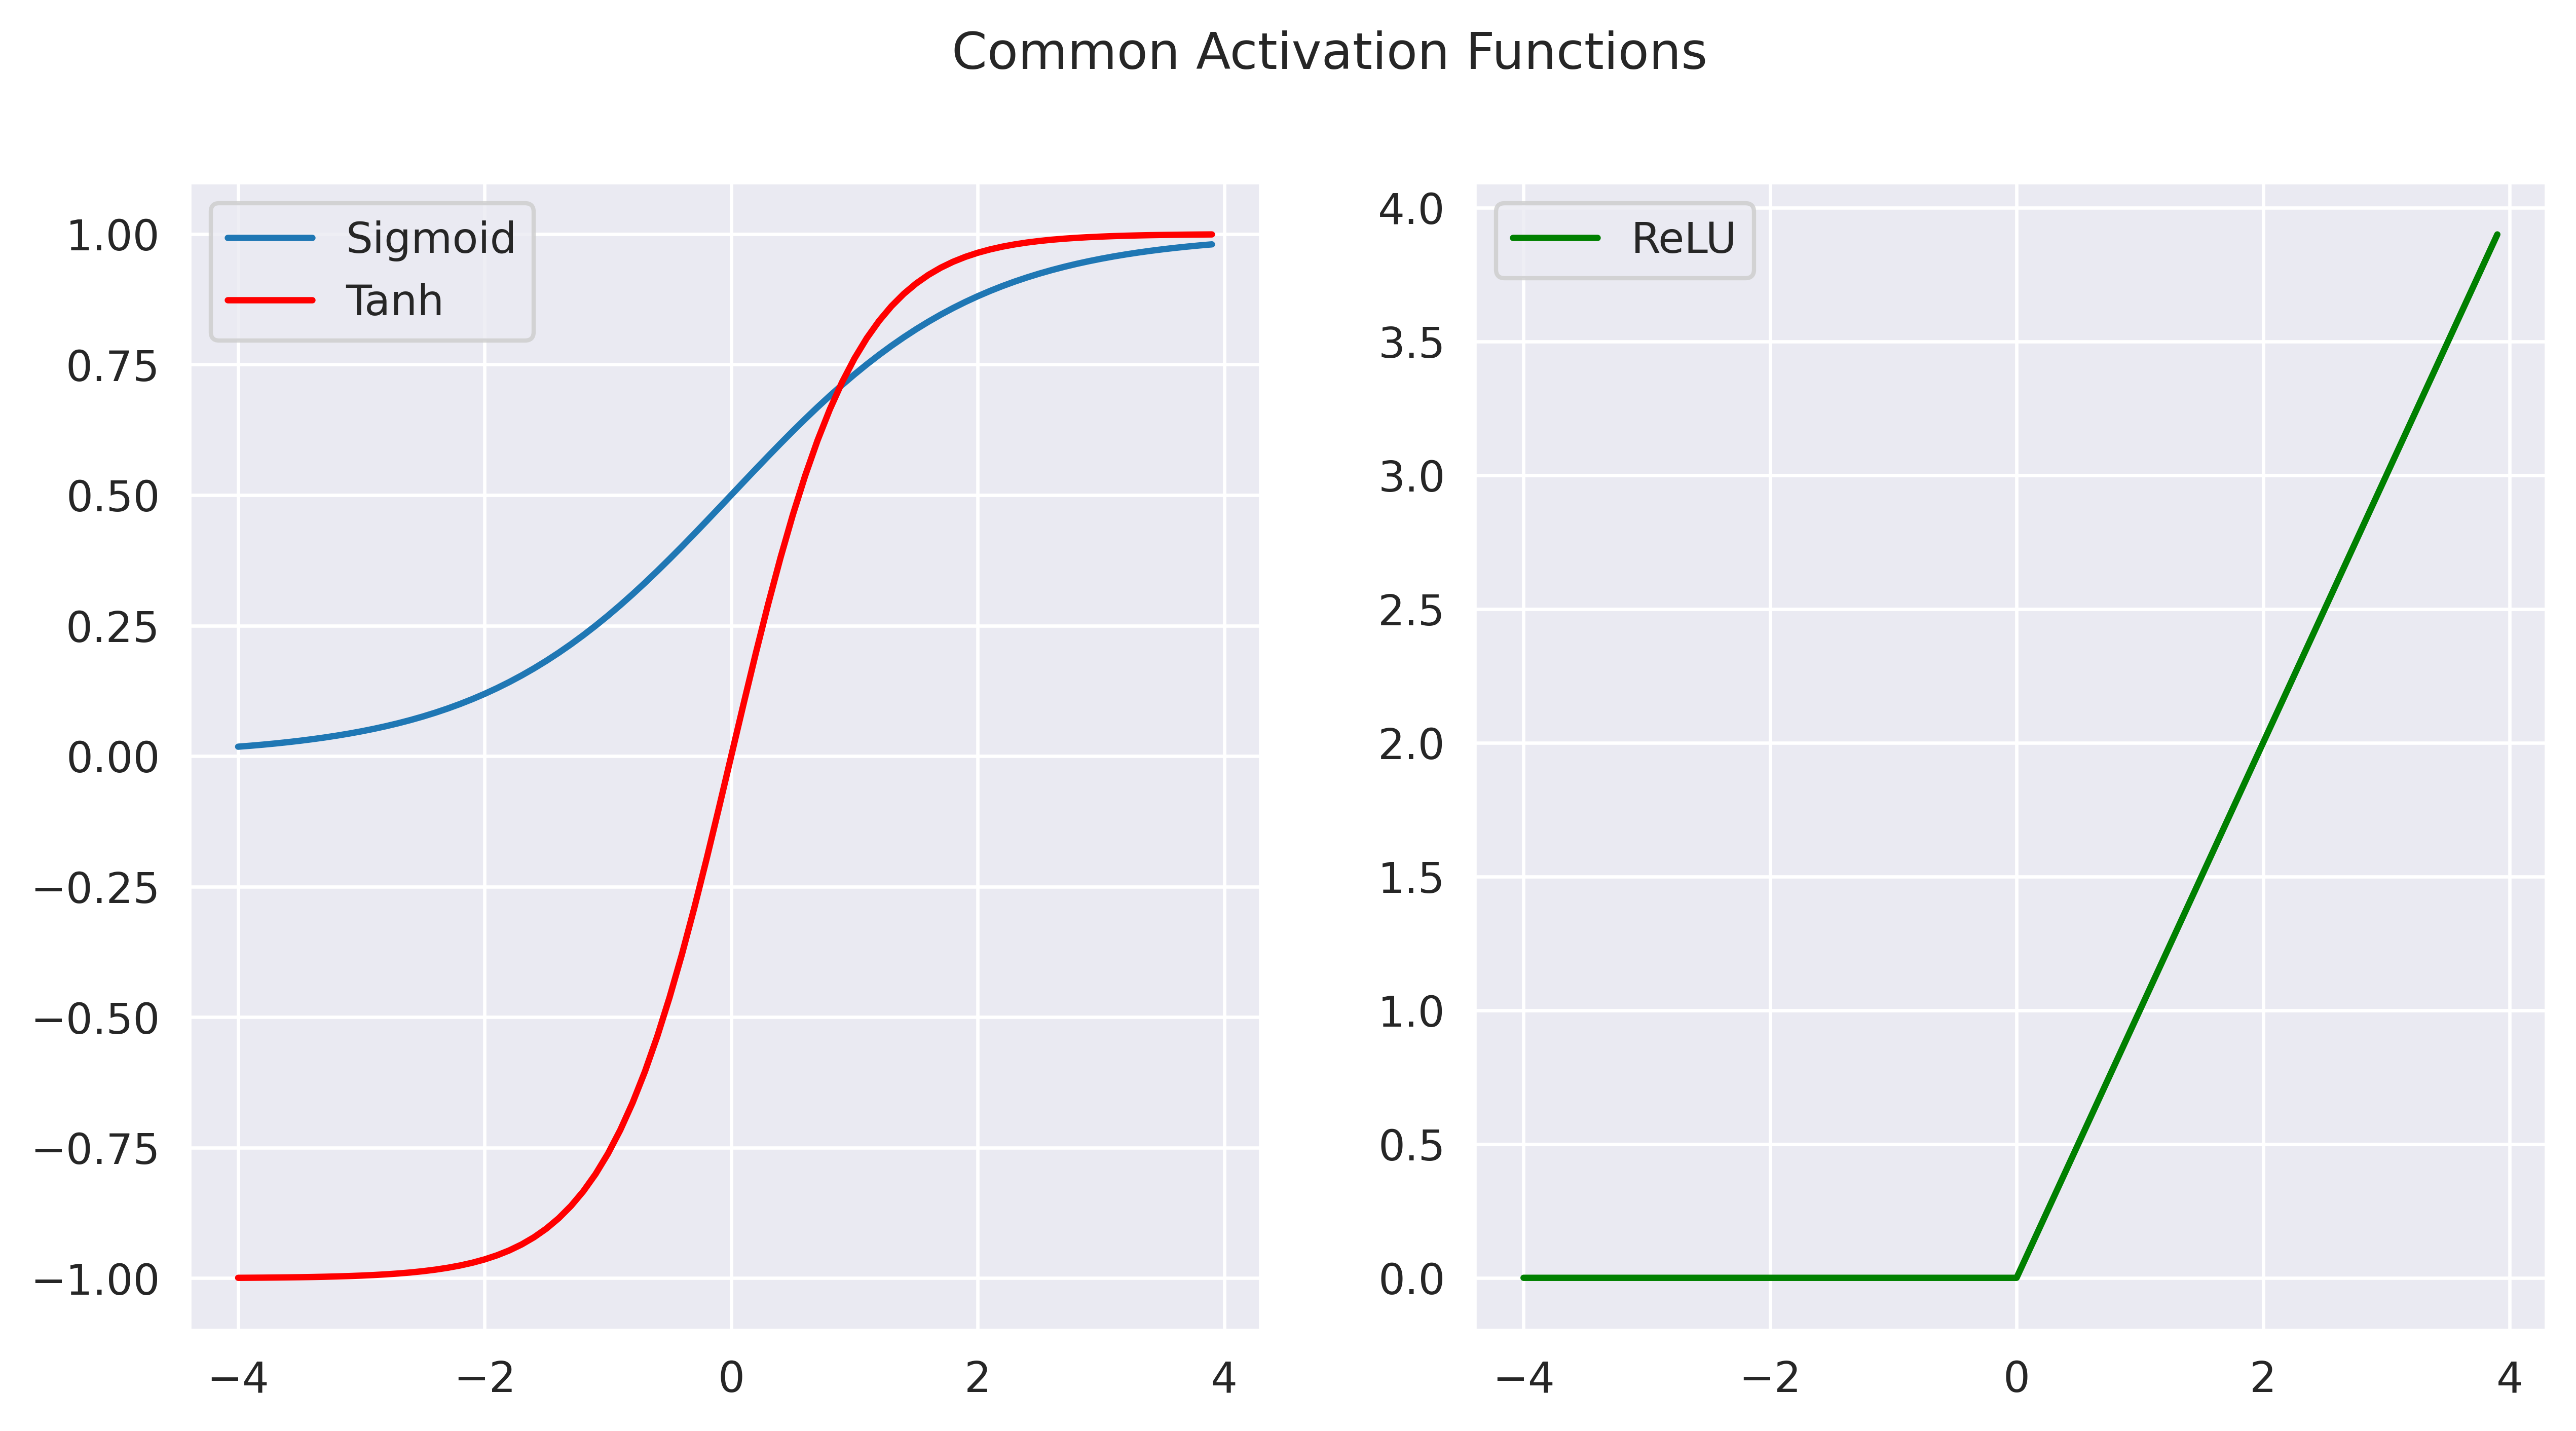
\includegraphics[width=\linewidth]{Chapters/Figures/sigmoids.png}
    \caption[Activation-Functions]{Plotted are three common activation functions: sigmoid, tanh, and ReLu.}
    \label{fig:ActivationFunctions}
\end{figure}

\subsubsection{ReLU}
The \textbf{Re}ctified \textbf{L}inear \textbf{U}nit activation function, or ReLU has become an important staple of machine learning. The activation function, $ f(x) $, is defined as the following:
\begin{equation}
f(x)=
\begin{cases}
    0 & \text{if } x <= 0 \\
    x & \text{if } x > 0
\end{cases}
\end{equation}

\noindent ReLU is important because it provides a much greater range in values. Whereas the sigmoid and tanh activation functions saturate around 4, ReLU never saturates for linear values. Additionally, ReLU is simple to calculate and tends to help neural networks converge quickly. Arguably thier most major benefit is the reduced likelihood of creating a vanishing gradient. Further, because ReLU returns 0 for any negative value fed foward into the node, many ReLU activation functions in a given layer help lead to sparser layers, reducing the overall complexity of the model and helping prevent overfitting.


\begin{figure}
    \centering
    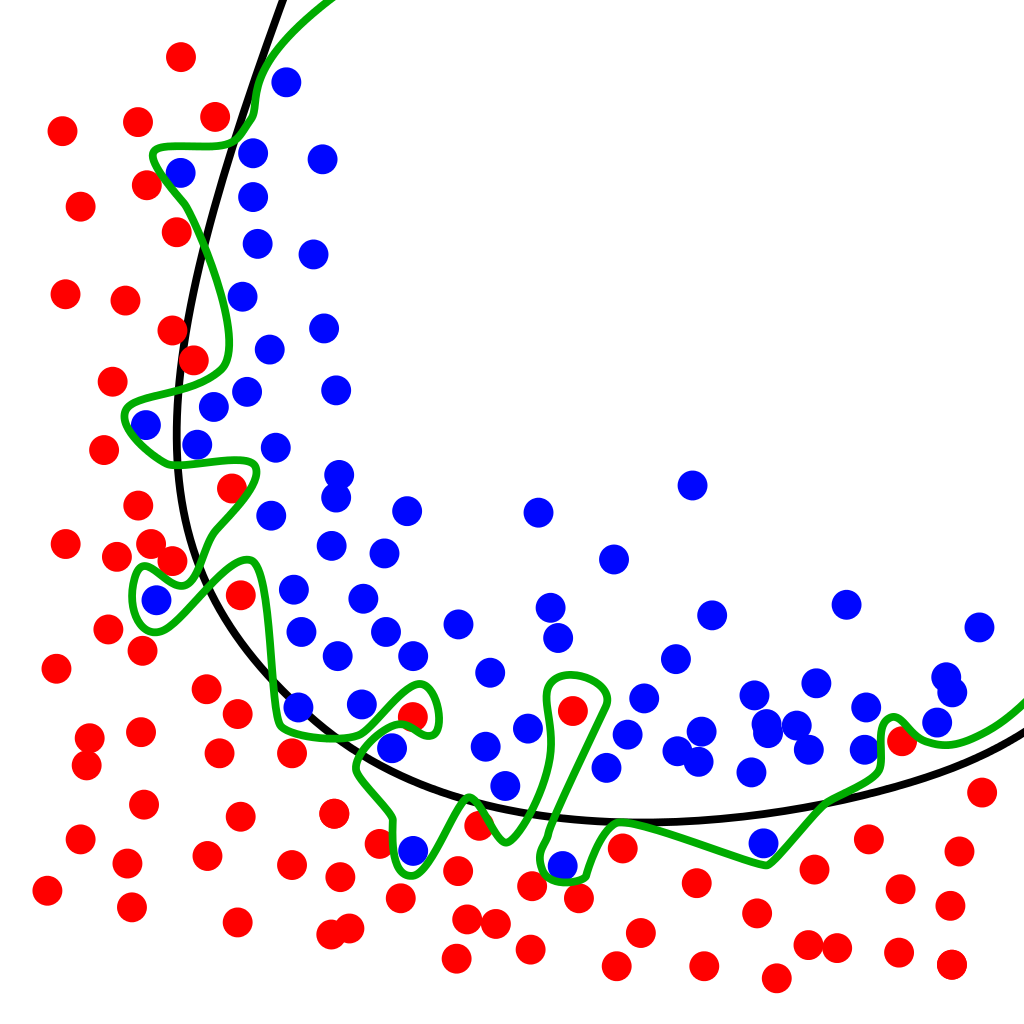
\includegraphics[width=.5\linewidth]{Chapters/Figures/overfitting.png}
    \caption[Overfitting]{The green curve represents a model that is overfitting the data in a binary classification problem. Although it makes perfect predictions for the training data in this figure, the model will not generalize well. Introducing biases and including dropout layers in neural networks are strategies to prevent overfitting.}
    \label{fig:overfitting}
\end{figure}


With the input nodes dotted with the weights, the baises added, and then the activation function calcuated for each node, we arrive at the final final for the first hidden layer. Mathematically, $ h_\nu^{(1)} = \sigma\left( x_\mu W_\nu ^\mu + b_\nu \right) $. This process is now repeated, only with the starting layer $ h_\nu^{(1)} $ and the output
$ \hat{y} = \sigma \left( h_\nu W_\kappa ^\nu + b_\kappa \right)$ is the final output of the neural network. The equations for each step as well as the dimensionality of each layer can be found in Figure \ref{fig:simpleNN}.

\begin{figure}[h!]
    \centering
    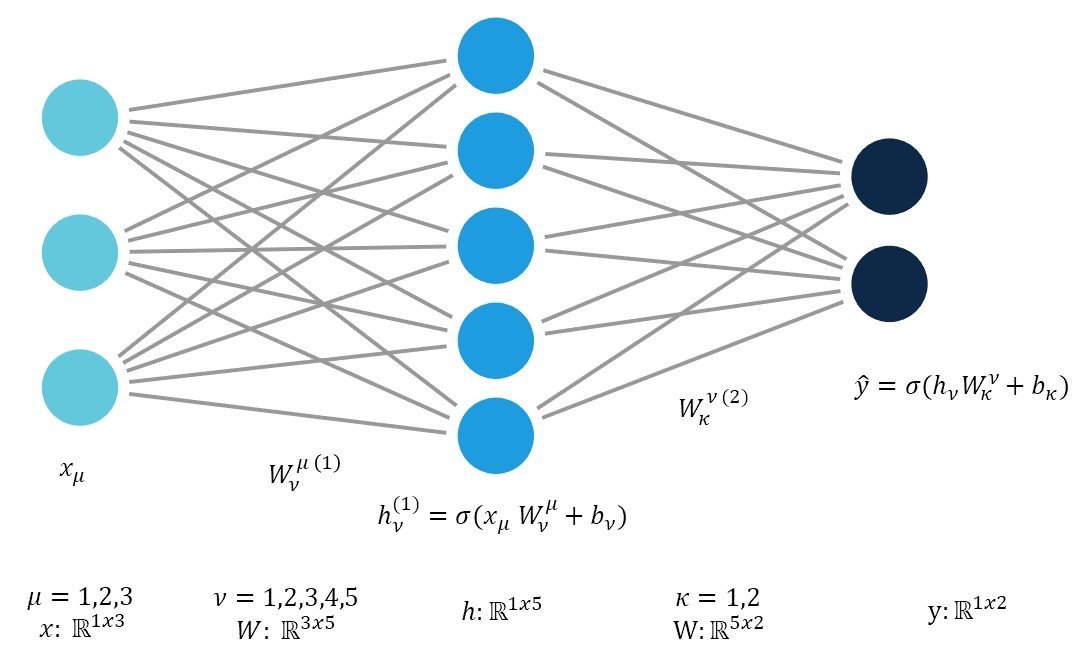
\includegraphics[width=\linewidth]{Chapters/Figures/einstein_NN.png}
    \caption[Neural Network Example]{Figure first made by me for my website}
    \label{fig:simpleNN}
\end{figure}

\subsection{Loss Metrics and Regularization}
It is necessary to evaluate the quality of every prediction the neural network makes in order to update the netork parameters. The measure of the error in one prediction is referred to as the \textit{loss}, and the summed total of all the errors in predictions is called the \textit{cost}. For regression problems, the two most common cost functions are the mean squared error and the mean absolute error. These are also referred to as the L2 and L1 costs, respectively, and defined as:

\begin{align}
    \label{eqn:lossFunctions}
    \text{L1 Cost} &= \frac{1}{n} \sum \left( \hat{y} - y \right) \\
    \text{L2 Cost} &= \frac{1}{n} \sum \left( \hat{y} - y \right)^2
\end{align}

\noindent where $ n $ is the number of training sampels. The equation for updating the weights under L2 regularization is as follows:
\begin{equation}
    W := (1-\alpha \lambda)W - \frac{\partial J}{\partial W}  
\end{equation}

\noindent where $\alpha$ is the learning rate, $\lambda$ is the regularization hyper-parameter, and J is the cost. L2 regularization is often referred to as weight decay. Every iteration the weights are pushed closer to zero due to the multiplicatiion of the weights by a value $<1$. For L2, the equation for the cost is:

\begin{equation}
\text{L2 cost} = \sum (y_i - y)^2 + \lambda \sum (W)^2
\end{equation}

L1 regularization is just the same as above, but with an absolute value for the regularization term instead of a square. L1 is known as LASSO (least absolute shrinkage and selection operator), because it shrinks the less important features' coefficients to zero. This is because for small values $abs(w)$ is a much stiffer penalty than $w^2$. Thus, L1 is thus a good choice when you have a ton of features.

% \noindent Explicitly, for one component of the hidden layer:

% \begin{align}
%     h_j &= \sigma(w_{1j}x_1 + w_{2j}x_2 + w_{3j}x_3 + w_{4j}x_4 + w_{5j}x_5 + b_j) \\
%         &= \sigma\Big(\sum_{i=1}^{i=5}w_{ij}x_{i} + b_j\Big)
% \end{align}


\noindent The process can be repeated ad-nauseam for networks with more layers.

\subsection{Backpropagation}
Backpropagation is the process of updating all the trainable parameters of the machine learning model, including weights, biases, and any other trainable parameters. The partial derivative require repeated use of the chain rule. Representing the above neural network as a functional yields the equation:

% \begin{equation}
%     \hat{y} = \sigma\left( g \left( f() \right) \right)
% \end{equation}
% \noindent This would be a network with inputs $(x, y)$, two hidden layers ($ f $  and $ g $ ), and an output with activation function sigma. Let's say the loss is the RMS loss. Thus,

\begin{equation}
    \label{eqn:functional}
    \hat{y} = \sigma \left( h_\nu ^{(1)} \left( x_\nu \right) \right)
\end{equation}

\noindent where the the output layer $ \hat{y} $ is a function of the hidden layer, $ h_\nu ^{(1)} $ which in turn is a function of the input layer $ x_\mu $. Consider the L2 loss (\ref{eqn:lossFunctions}). Note that the loss function is a function of the previous functional (\ref{eqn:functional}). To see how much to shift the weights, calcuate the gradients for each layer. The first partial derivative is trivial:

\begin{equation}
    \frac{\partial J}{\partial J} = 1
\end{equation}

\noindent For the next layer (the output layer):

\begin{equation}
\frac{\partial \hat{y}}{\partial J} = \frac{\partial J}{\partial J}\frac{\partial \hat{y}}{\partial J}
\end{equation}


\noindent For the next nested-function (the sigmoid):

\begin{equation}
\frac{\partial J}{\partial \sigma} = \frac{\partial J}{\partial \hat{y}} \frac{\partial \hat{y}}{\partial \sigma}
\end{equation}


\noindent The next layer is the hidden layer before the activation function. For simplicity it will be referred to as $ g $ where $ g = x_\mu W_\nu ^\mu + b_\nu $.  

\begin{equation}
    \frac{\partial J}{\partial g} = \frac{\partial J}{\partial \hat{y}} \frac{\partial \hat{y}}{\partial \sigma} \frac{\partial \sigma}{\partial g}
\end{equation}


\noindent Next layer is the input layer, $ X_\mu $ has no trainable parameters, so the process for this network architecture is complete. If there were more hidden layers, the chaining rule would continue by multiplying the gradient calculated in the previous step by the gradient of the next layer with respect to the previous layer (towards the input layer). 

% \begin{equation}
%     \frac{\partial L}{\partial f} = \frac{\partial L}{\partial \hat{y}} \frac{\partial \hat{y}}{\partial \sigma} \frac{\partial \sigma}{\partial g} \frac{\partial g}{\partial f}
% \end{equation}

\subsection{Concrete Example}

Finally, we will repeat the backpropogation process of updating the weights for the previous example as explicitly as possible. Consider again the functional $ \hat{y} $ in equation (\ref{eqn:functional}) and the L2 loss in equation (\ref{eqn:lossFunctions}), rewritten here as $ L $ . To determine how do shift the weights in the function, want to know $\frac{\partial J}{\partial W}$, where $ W  $ is short for $ W_\kappa ^{\nu (2)} $, the weight matrix connected to the second layer (the output layer). 

\begin{align}
L = \frac{1}{m}\sum(\hat{y} - y)^2 \\
\end{align}

\noindent As before, the first partial derivative is trivial

\begin{equation}
    \frac{\partial J}{\partial J} = 1
\end{equation}

\noindent and the next partial derivative is also strait-foward:

\begin{equation}
\frac{\partial J}{\partial \hat{y}} = 2(\hat{y} - y )
\end{equation}

\noindent Applying the chain rule yields:

\begin{equation}
\label{eqn:dldy}
\frac{\partial J}{\partial \hat{y}} = \frac{\partial J}{\partial J}\frac{\partial J}{\partial \hat{y}} \\
= 1 \cdot 2(\hat{y} - y )
\end{equation}

\noindent The next required term in the chain is the derivative of the loss with respect to the sigmoid:

\begin{equation}
\frac{\partial J}{\partial \sigma} = \frac{\partial J}{\partial \hat{y}} \frac{\partial \hat{y}}{\partial \sigma}
\end{equation}

\noindent We already found the first term (\ref{eqn:dldy}), and the second term in trivial.

\begin{equation}
    \frac{\partial \hat{y}}{\partial \sigma} = 1 \\
    \implies \frac{\partial J}{\partial \sigma} =  \frac    {\partial J}{\partial \hat{y}} \frac{\partial \hat{y}}  {\partial \sigma} \\
    = 2(\hat{y} - y ) \cdot 1
\end{equation}

\noindent At this point, we have the derivative $ \frac{\partial J}{\partial \sigma} $ for the $ \sigma $ in the final layer $ \hat{y} = \sigma \left( h_\nu W_\kappa ^\nu + b_\kappa \right) $. The next derivative in the chain will be $ \frac{\partial J}{\partial g} $ where $ g = h_\nu W_\kappa ^\nu + b_\kappa $ as before. Continuing the chain,

\begin{equation}
\frac{\partial J}{\partial g} = \frac{\partial J}{\partial \hat{y}} \frac{\partial \hat{y}}{\partial \sigma} \frac{\partial \sigma}{\partial g}
\end{equation}

\noindent where

\begin{align}
\sigma(g) &= \dfrac{1}{1 + e^{-g}} \\
\implies \frac{\partial \sigma}{\partial g} &= \sigma(g)(1 - \sigma(g))
\end{align}

\noindent Combining these previously calculated terms yields:

\begin{equation}
\frac{\partial J}{\partial f} = 2(\hat{y} - y ) \cdot 1 \cdot  \sigma(z)(1 - \sigma(z))
\end{equation}

Now comes the good part. Recall that the trainable parameters in the network are the weights and biases (W and b). The next step will is to calculate the gradients with respect to each, which in turn will be used to update the paramters.

\begin{equation}
\frac{\partial J}{\partial W} = \frac{\partial J}{\partial g}\frac{\partial g}{\partial W} = \frac{\partial J}{\partial \hat{y}} \frac{\partial \hat{y}}{\partial \sigma} \frac{\partial \sigma}{\partial g} \frac{\partial g}{\partial W}
\end{equation}

\noindent The last partial in the chain is

\begin{equation}
\frac{\partial g}{\partial W} = W
\end{equation}


\noindent So,

\begin{equation}
\frac{\partial J}{\partial W} = 2(\hat{y} - y ) \cdot 1 \cdot  \sigma(z)(1 - \sigma(g)) \cdot W
\end{equation}

\noindent For the baises,

\begin{align}
\label{eqn:dLdW}
\frac{\partial J}{\partial b} &= \frac{\partial J}{\partial g} = \frac{\partial J}{\partial \hat{y}} \frac{\partial \hat{y}}{\partial \sigma} \frac{\partial \sigma}{\partial g} \frac{\partial g}{\partial b} \\
\frac{\partial g}{\partial b} &= 1 \\
\implies \frac{\partial J}{\partial b} &= 2(\hat{y} - y ) \cdot 1 \cdot  \sigma(g)(1 - \sigma(g)) \cdot 1
\end{align}

Note that $ W $ is actually $ W_\kappa ^{\nu (2)} $, a matrix of weights, and b is actually $ b_\kappa $, a row vector of biases. Thus, the above equation (\ref{eqn:dLdW}) is just the partial derivative for one term in the weight matrix or bias vector. Repeating the process for each term in the matrix W and vector b yields the gradients $ \nabla_w L $  and $ \nabla_B L $, which represent the gradient of the loss function with respect to the weights and biases, respectively. This is the origin of the term, ``gradient descent,'' an optimization algorithm discussed in the next section. This was just the process to calculate the gradients need to update weights for the final layer, but one can see how continuing the process of chaining partial derivatives will yield the gradients for earlier layers in the network.

\section{Optimizers}
Having calculated all the gradients via backpropagation, the weights and biases of the network can now be adjusted. The general idea of gradient descent relies on the fact that the gradient of a function points in the direction of greatest increase. Thus, to optimize the network ---which is equivalent to finding the parameters that minimize the value of the loss function--- the weights and biases are updated by shifting their values in the opposite direction of the gradient of the loss function with respect to the weights, $ \nabla_w L $ . Gradient descent is the core principle of machine learning; this efficient algorithm for systematically updating model-parameters, made it possible to develop deep neural networks and train them with large datasets. Several improvements have been made to gradient descent since its inception \cite{cauchy-orig-grad-descent}, with the state of the art being AdamW \cite{AdamW-orig}. In this section, several optimization algorithms are introduced in order to provide context for Adam, the optimizer used for training our model. In the previous section, the gradients for the weights and biases were written explicitely. For simplicity, the variable $ \theta $ is introduced to refer to either parameter. As before, $ J(\theta) $  is the cost function; it could be the L1 or L2 cost, or any other differentiable measurement of fit quality.

\subsubsection{Gradient Descent}
Vanilla gradient descent \cite{gradient-descent-rev-article} updates the parameters in the following way:

\begin{equation}
    \label{batch-grad-descent}
    \theta := \theta - \eta \cdot \nabla_\theta J(\theta)
\end{equation}

\noindent Here (\ref{batch-grad-descent}), $ \eta $ is a \textit{hyperparameter} known as the learning rate. A hyperparameter is a user-defined parameter that must be chosen before the training process begins; it is not a trainable parameter. One limitation to gradient descent is the need for the entire cost $ J $ to be calculated. For large datasets, this can become impractical. Two common variants are batch gradient descent and stochastic gradient descent (SGD). In the former, the training set is divided into batches and the gradient is updated after each batch. One iteration through all the batches is called an \textit{epoch}. In the latter, the gradient is calculated using the loss function instead of the cost function, i.e. the gradient is calculated and the parameters are updated after each training sample. Both methods greatly reduced training time with the help of optimized, parallel computing \cite{stoch-grad-desc-parallel}. By updating the parameters after every training sample, SGD will move in the direction of the true gradient. The major limit to these methods, however, is the fixed learning rate \cite{grad-desc-limits}. If the learning rate, $ \eta $ is too large, the algorithm will be unstable and ``bounce'' around the global minimum of the cost function. If $ \eta $ is too small, the algorithm will, at best, take a long time to train, and at worst, end up stuck in a local minimum. 

\subsubsection{Stochastic Gradient Descent with Momentum}
Compared to regular SGD, stochastic gradient descent with momentum \cite{grad-desc-with-mom-orig} can greatly reduce the time to convergence. The general idea is to add a fraction of the previous parameter update to the current update. The exponential moving average (EMA) is an averaging of points within a period that puts greater weight on more recent points\footnote{In contrast a simple moving average treats each point as equally significant}. Here, $ S_t $ is the $ t^{th} $  value in the sequence S, and $ V_t $ is the $ t^{th} $  value in the new exponential moving averaged sequence, $ V $ .

% \begin{align}
%     % \label{eq:SGD}
%     & V_1 = \beta V_0 + \left(1 - \beta \right) S_1 \\
%     & V_2 = \beta V_1 + \left(1 - \beta \right) S_2 \\
%     & ...
% \end{align}
\begin{equation}
    \label{eq:SGD-w-momentum}
    V_t = \beta V_{t-1} + (1 - \beta)S_t
\end{equation}

\noindent where $ \beta \epsilon [0,1]$, a hyperparameter which partly defines how much weight the previous $ 1/(1-\beta) $ terms of S contribute\footnote{Typically 0.90 is a good starting point}. EMA's are common in market forecasting, so often $ S_t $  is the price at time $ t $. The continuous update for SGD with momentum is as follows:

\begin{align}
    V_t &= \beta V_{t-1}  + \left( 1 - \beta \right) \nabla_\theta J \left( \theta \right)\\
    w &= W - \alpha V_t
\end{align}


Here, $ \alpha $  is the learning rate, as always. To be clear, $\nabla_w L$ is the gradient of the loss function with respect to the weights. Note that the cost function $ J(\theta) $ may instead be the loss function $ L(\theta) $ if updates are performed after each training sample (i.e.~a batch size of one). SGD with momentum tends to perform better than SGD because it gives a closer estimate of the full gradient from the batch than SGD. Additionally, the momentum helps push the update through ravine-shaped local minima in the correct direction, whereas SGD tends to oscillate back and forth along the ravine's steeper dimension \cite{qian1999momentum}.

\subsubsection{RMS Propagation}
RMS prop is another variant of SGD to improve convergence speed \cite{improving-rprop} \cite{adagrad} \cite{2017marginal-adagrad}. Once again, the idea is to dampen oscillations in directions where you are close to the minimum, and accelerate movement when you are far from the minimum. Here, we keep a moving average of the squared gradients for each weight. As before, $\nabla_\theta L$ is the gradient of the cost with respect to weights.

\begin{align}
    \label{eqn:RMS_Prop}
    & S_{k+1} = \beta S_k + (1 - \beta)(\nabla_\theta L \cdot \nabla_\theta L) \\
    & \theta_{k+1} = \theta_k - \alpha \frac{\nabla_\theta L}{\sqrt{S_{k+1}} + \epsilon}
\end{align}

\subsubsection{Adaptive Moment Estimator}
Adam is a combination of RMS prop and SGD with momentum. It uses the squred gradients to scale the learning rate (like RMS prop), and it uses a moving average of the gradient (like SGD with momentum). It's 80,000 ciations in the 6 years since its publication gives some indication of the importance and power of this algorithm \cite{orig-ADAM-paper}.

\begin{align} 
    \begin{split} 
    m_t &= \beta_1 m_{t-1} + (1 - \beta_1) g_t \\ 
    v_t &= \beta_2 v_{t-1} + (1 - \beta_2) g_t^2 
    \end{split} 
\end{align}


\section{Batch normalization}

Batch normalization is a way to make your network more robust to covariance shift\footnote{Covariate shift is a type of dataset shift where the distribution of training data differs from that of testing, or in this context, batch to batch.} \cite{batch-norm-orig}  \cite{batch-norm-conference}. For example, if you train your cat vs. not cat identifier with only images of black cats, your network won't make good predictions when it comes to orange cats.

The idea is to normalize each hidden layer, similar to how you normalize the input dataset. However, whereas with normalization of training data centers the dataset around a mean of zero and STD of 1, the mean and variance of the batch normalization are trainable/learnable parameters.

Normalize input data i like:


\begin{equation}
    Z_{norm}^{(i)} = \frac{x_i-\mu}{\sqrt{\sigma^2-\epsilon}}
\end{equation}


Normalize the values for hidden layer l like:

\begin{equation}
\widetilde{Z}_i = \gamma Z_{norm}^{(i)} - \beta
\end{equation}

You can see that if $\sqrt{\sigma^2 + \epsilon}$ and $\gamma = \mu$, you get the first equation, i.e. you're normalizing the hidden layer in the same way as the input layer. You generally don't want to do this, however, because if you're normalizing everything to be centered around zero, your activation function will be mostly focused on the linear regime of the sigmoid.

The structure of implementing batch normalization looks something like this:

$$\text{first pass: } x \cdot \theta^T \rightarrow z$$
$$\text{batch normalize: } z \rightarrow \widetilde{z}$$ 
$$\text{apply activation function: } g(\widetilde{z}) = a$$
$$\text{second pass: } a \cdot \theta^T$$     
etc.

Note, this is for one mini-batch, so $x$ is the $i^{th}$ mini-batch. Normalizing the hidden layers for each batch means that later hidden layers don't have to adapt as much to the earlier hidden layers. This means that the later layers can do a better job tuning themselves a little more independently of the other layers, and it speeds up the learning process. Note, because you're scaling each mini-batch $(z \rightarrow \widetilde{z})$, you add a little bit of noise, which is a little bit of regularization. But don't use batch-norm as a form of regularization. That's not its purpose.

\section{Covolutional Neural Networks}
Convolution is a mathematical operation for combining two functions, the result of which is a third function revealing the effect of the second function on the first \cite{Boas-mathmethods}. The convolution of two continuous functions, $ f $ and $ g $, is a special type of integral transformation. The result is the integral of the product of $ f $ and the shifted inverse of $ g $, where $ f $ can be thought of as the input function and $ g $ is often referred to as the kernel.

\begin{equation}
    f \otimes g = \int_{-\infty}^{\infty} f(\tau)g(t-\tau) \,d\tau 
\end{equation}

\noindent The variable $ i $ (no relation to the imaginary number) is represents the weighted-shift in the function $ g(\tau) $. Different values of $ i $ emphasize different parts of the other function, $ f(\tau) $.  

In computer science, convolutions are an important and powerful tool for signal and image processing \cite{1dconv-NN-survey} \cite{deepCNNforImages}. Because images and signals ---which can be thought of as a 1D image --- are comprised of a discrete number of points (e.g.~pixels), a modified foruma is required. The convolution of the signal $ f $ with the kernel $ g $ can be written as \cite{cornell-convs}:

\begin{equation}
    \label{eqn:cs-1dconv}
    f \otimes g = \sum_{j=1}^m g(j) \cdot  f(i-j+m/2)
\end{equation}

\noindent Here (\ref{eqn:cs-1dconv}), $ m $ is the length of the kernel $ g $, and $ i $ and $ j $ are hyperparameters. To demonstrate visually, consider a simple, example absorption spectrum with only 10 data points (\ref{fig:conv-ex-spectrum}).

\begin{figure}[h!]
    \centering
    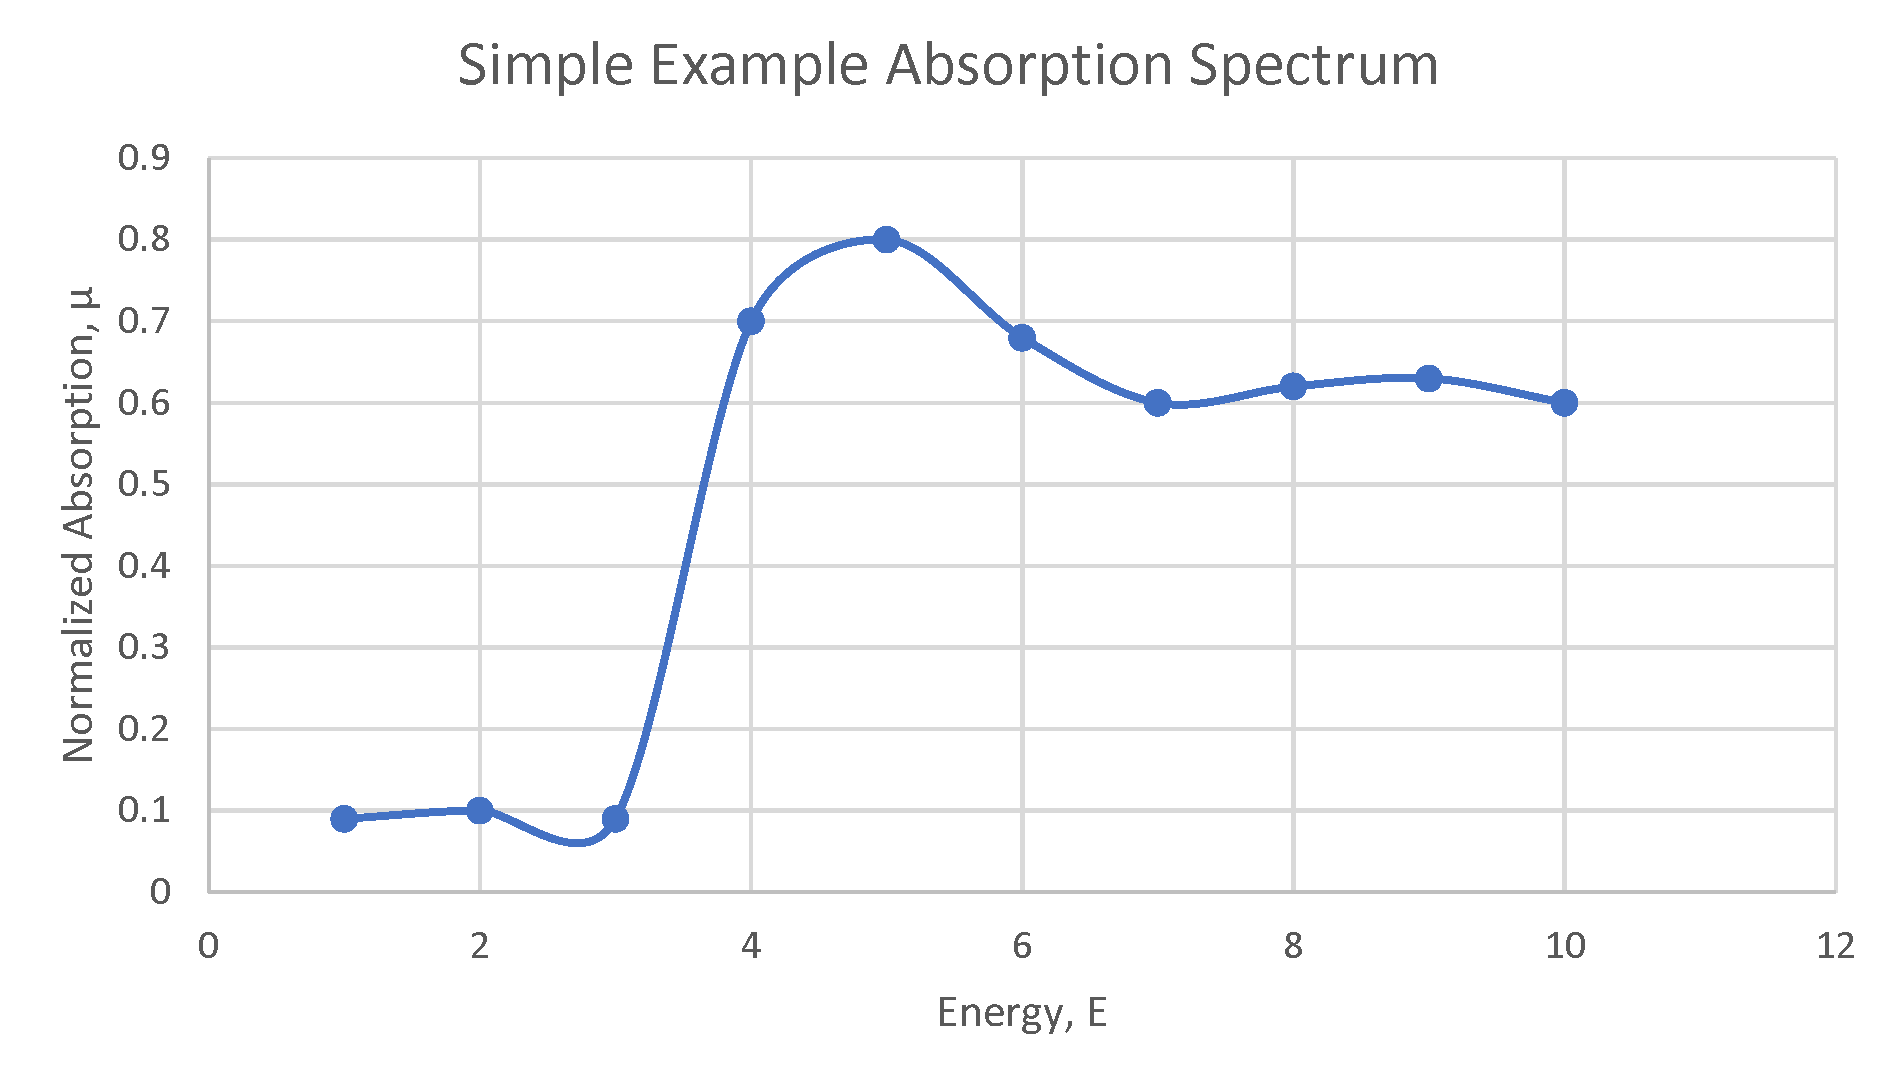
\includegraphics[width=.75\linewidth]{Chapters/Figures/conv-example.png}
    \caption[Toy Absorption Spectrum]{A simple abosrption spectrum for demonstration purposes.}
    \label{fig:conv-ex-spectrum}
\end{figure}
 
\noindent Each data point, $ (E, \mu) $ in the spectrum is described as a feature vector, where the feature is the the energy value for a given point $ (E, \mu) $. The vector is depicted in (\ref{conv-squares}) with zeros padded on both sides. Additionally, consider a kernel, $ g $  

\begin{table}[h!]
    \centering
    \begin{tabular}{c|c|c|c|c|c|c|c|c|c|c|c|c|}
    \cline{2-13}
    \textit{f} = & 0 & .09 & .10 & .09 & .70 & .80 & .68 & .60 & .62 & .63 & .60 & 0 \\ \cline{2-13}
    \end{tabular}
    \label{conv-squares}
\end{table}

\begin{table}[h!]
\centering
    \begin{tabular}{lccc}
    \cline{2-4}
    \multicolumn{1}{l|}{\textit{g} =} & \multicolumn{1}{c|}{.1} & \multicolumn{1}{c|}{.1} & \multicolumn{1}{c|}{.1} \\ \cline{2-4}                 
    \end{tabular}
\end{table}

\noindent The convolution works by mutliplying each element in the input vector $ f $ by the corresponding element in the kernel $ g $ and summing the results. The kernel then moves to be centered around the next element in $ f $. One way to think about this process is a kernel or filter sliding over an input signal. Applying the kernel $ g $ onto the first index of $ f $ yields: 

\begin{table}[h!]
    \centering
    \begin{tabular}{|c|c|c|c|c|c|c|c|c|c|c|c|}
    \hline
    0  & .09 & .10 & .09 & .70 & \multicolumn{1}{c|}{.80} & \multicolumn{1}{c|}{.68} & \multicolumn{1}{c|}{.60} & .62 & .63 & .60 & 0 \\ \hline
    .1 & .1  & .1  &     &     &                          &                          &                          &     &     &     &   \\ \hline
    \end{tabular}
\end{table}
$$ 
h(1) = (0)(.1) + (.09)(.1) + (.10)(.1) = 0.019
$$

\noindent where $ h(1) $ is 1st index of the resulting vector. For the next point, the kernel shifts to be centered around it. 

\begin{table}[h!]
    \centering
    \begin{tabular}{|c|c|c|c|c|c|c|c|c|c|c|c|}
    \hline
    0 & .09 & .10 & .09 & .70 & \multicolumn{1}{c|}{.80} & \multicolumn{1}{c|}{.68} & \multicolumn{1}{c|}{.60} & .62 & .63 & .60 & 0 \\ \hline
      & .1  & .1  & .1  &     &                          &                          &                          &     &     &     &   \\ \hline
    \end{tabular}
\end{table}

$$ 
h(2) = (.09)(.1) + (.10)(.1) + (.09)(.1) = 0.028
$$

\noindent The final resulting vector is:

\begin{table}[h!]
    \centering
    \begin{tabular}{c|c|c|c|c|c|c|c|c|c|c|}
    \cline{2-11}
    \textit{h} = & .019 & .028 & .089 & .159 & .218 & .208 & .190 & .185 & .185 & .123 \\ \cline{2-11} 
    \end{tabular}
\end{table}

\begin{figure}[h!]
    \label{fig:conv-res-spectrum}
    \centering
    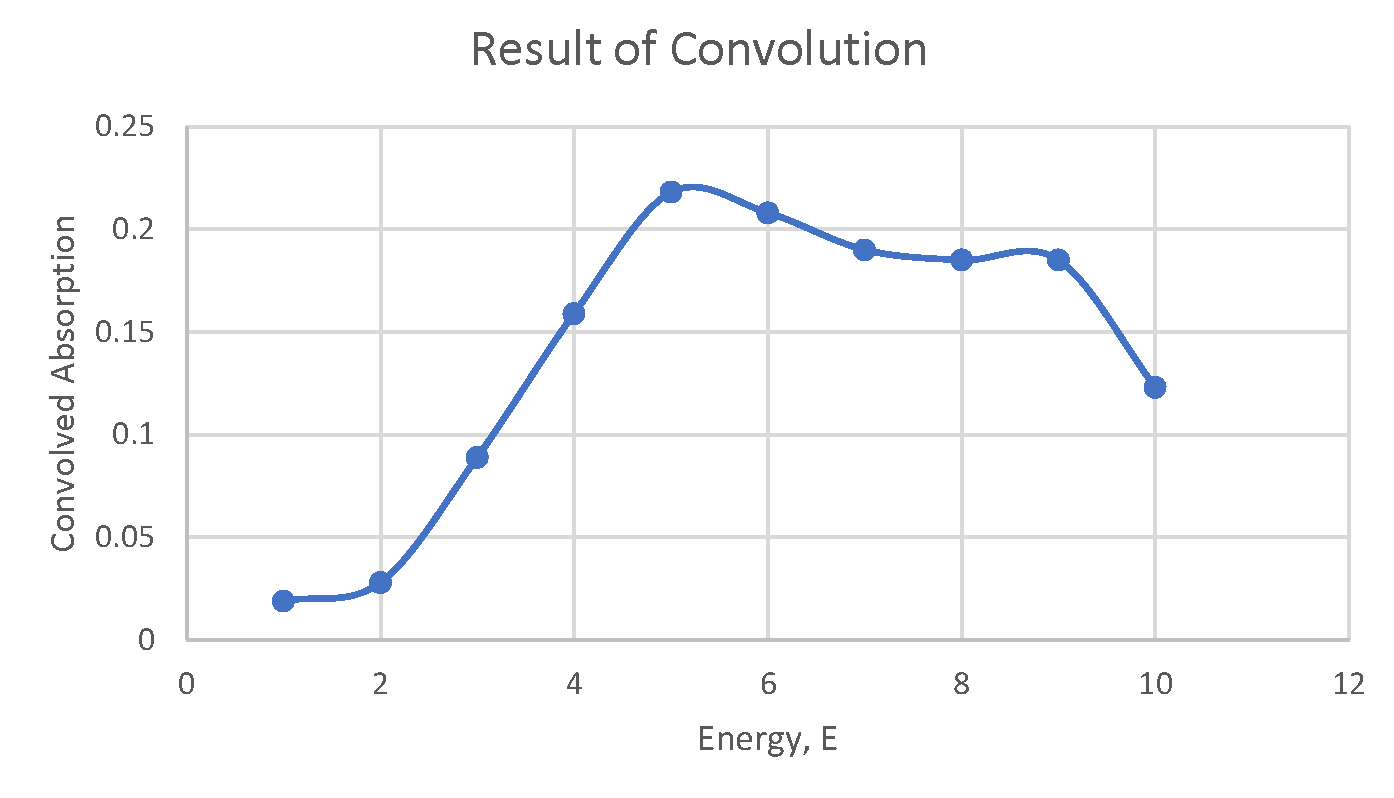
\includegraphics[width=.75\linewidth]{Chapters/Figures/conv-example-res.png}
    \caption[1D Convolution Result]{The result of the 1D convolution of kernel $ g = (.1, .1, .1) $  on the spectrum in Figure \ref{fig:conv-ex-spectrum}.}
\end{figure}

The toy example was chosen to demonstrate the basics of a 1D convolution. In this example, the input spectrum was a vector of length ten and the kernel of length three. In the context of applying a 1D convolution to a neural network, the size of the input vector is the cardinality of the hidden layer directly preceding the convolutional layer. Often the hidden layer's output, represented as a vector, is reshaped into an n-dimensional tensor before applying the convolution. To apply a 1D-convolution to a Tensor of rank $ n $, simply apply the convolution to each of the n-vectors separately, ensuring to pad the ends of each vector with zeros. Layers with dimensionality greater than one can be ``un-raveled''. Alternatively, the layers of each dimension can be truncated or ``pooled'' by averaging the layers that are stacked on one another (or taking the max of each layer) until the desired dimensionality is achieved. A common way to achieve this is with a max pooling layer or an average pooling layer. Max pooling and average pooling layers also have the additional benefit of downsampleing the feature space, tending to make the network more robust to slight variations in the position of features in the input image or signal. This is referred to as ``local translation invariance'' \cite{local-translation-invariance}.

Another important possible change, in the above example, we ``slid'' the kernel across the input spectrum one point at a time. This is referred to as a stride size of one. The stride could be any integrer less than the length of the input vector $ f $, though in practice, typically a stride lengths tend to be one or close to one. Lastly, in the above example, we only applied one convolutional kernel, or ``filter.'' In practice, many filters are applied sequentially. In the above example, the filter $ g = (.1, .1, .1) $ was simply decided upon \textit{a priori}. In practice, the values for each filter in the convolutional layer are initialized randomly or according to the specified initialization funciton. The default in Keras is Glorot Uniform. The values of each filter are trainable parameters which evolve to produce the best final prediction given the subsequent layers in the neural network.


\section{How to Train a Neural Network}
Here is the process for building a NN for cifar10Permalink.
You need to start with a simple model first. Pick some hype hyperparameters to see if you can overfit it (say, make the training set 1 - 10 images). If you can overfit it, then it means your code is working and your architecture makes sense. Next you can up the images to say 1000 and run a broad hyperparameter search. Afterward, run maybe 20 epochs and see how the training and validation loss are moving. If they both are going down, your architecture looks good. If not, start over.

Once it looks like your training loss is continuing to decrease but your validation loss plateaus, it’s time to start introducing regularization (say nn.Dropout(.5)) and data augmentation. This way you won’t continue to overfit the data and can keep dropping the validation loss.

I haven’t done it yet with the cifar10 set, but I suspect that you should build up a more complex architecture without regularization and make sure you can overfit it to death before tuning hyperparameters and introducing regularization.

If you start with a complex model with data augmentation and regularization you’ll never be able to tune the hyperparameters and find a good solution.

It’s best to put dropout layers after a ReLU activation and before an affine (nn.Linear()) layer


% \section{Autoencoders if they become useful}
% Talk about how autoencoders work. Give a nice broad explanation and really go into the math. Include some nice diagrams

% Here's \cite{ng2011sparse} a good source to read and model off of. Here \cite{Bhowick2019} is another paper that might be interesting to read. It's about getting noise-free data from the original data using an autoencoder. Neat idea, and could actually be very relevant because they're using geophysical data.



